
%(BEGIN_QUESTION)
% Copyright 2009, Tony R. Kuphaldt, released under the Creative Commons Attribution License (v 1.0)
% This means you may do almost anything with this work of mine, so long as you give me proper credit

This water level control system controls the level of water in a vessel by either adding ``make-up'' water to the vessel or by draining excess water out of it (but never both at the same time!).  The level transmitter outputs 4 mA with an empty tank and 20 mA with a full tank:
 
$$\includegraphics[width=15.5cm]{i03784x01.eps}$$

Assuming reverse action in the controller, determine the proper split ranges of the two control valves:

% No blank lines allowed between lines of an \halign structure!
% I use comments (%) instead, so that TeX doesn't choke.

$$\vbox{\offinterlineskip
\halign{\strut
\vrule \quad\hfil # \ \hfil & 
\vrule \quad\hfil # \ \hfil \vrule \cr
\noalign{\hrule}
%
% First row
Drain valve position & Controller output signal \cr
%
\noalign{\hrule}
%
% Another row
Fully shut (0\%) & ??? mA \cr
%
\noalign{\hrule}
%
% Another row
Wide open (100\%) & ??? mA \cr
%
\noalign{\hrule}
} % End of \halign 
}$$ % End of \vbox

% No blank lines allowed between lines of an \halign structure!
% I use comments (%) instead, so that TeX doesn't choke.

$$\vbox{\offinterlineskip
\halign{\strut
\vrule \quad\hfil # \ \hfil & 
\vrule \quad\hfil # \ \hfil \vrule \cr
\noalign{\hrule}
%
% First row
Make-up valve position & Controller output signal \cr
%
\noalign{\hrule}
%
% Another row
Fully shut (0\%) & ??? mA \cr
%
\noalign{\hrule}
%
% Another row
Wide open (100\%) & ??? mA \cr
%
\noalign{\hrule}
} % End of \halign 
}$$ % End of \vbox


\vfil 

\underbar{file i03784}
\eject
%(END_QUESTION)





%(BEGIN_ANSWER)

This is a graded question -- no answers or hints given!

%(END_ANSWER)





%(BEGIN_NOTES)

We need these two control valves to move in opposite directions, and we also need them to never be open at the same time (as that would waste water).  Thus, the type of split-range sequencing we need is {\it exclusive}.

\vskip 10pt

Given reverse action in the controller, the controller output will be low (toward 4 mA) when the water level is high.  Thus, we need the drain valve to be wide open at 4 mA and the make-up valve to be completely shut at 4 mA.  Thus, our split-ranging ``wedge diagram'' must look like this:

$$\includegraphics[width=15.5cm]{i03784x02.eps}$$

Translating this ``wedge diagram'' to table form:

% No blank lines allowed between lines of an \halign structure!
% I use comments (%) instead, so that TeX doesn't choke.

$$\vbox{\offinterlineskip
\halign{\strut
\vrule \quad\hfil # \ \hfil & 
\vrule \quad\hfil # \ \hfil \vrule \cr
\noalign{\hrule}
%
% First row
Drain valve position & Controller output signal \cr
%
\noalign{\hrule}
%
% Another row
Fully shut (0\%) & 12 mA \cr
%
\noalign{\hrule}
%
% Another row
Wide open (100\%) & 4 mA \cr
%
\noalign{\hrule}
} % End of \halign 
}$$ % End of \vbox

% No blank lines allowed between lines of an \halign structure!
% I use comments (%) instead, so that TeX doesn't choke.

$$\vbox{\offinterlineskip
\halign{\strut
\vrule \quad\hfil # \ \hfil & 
\vrule \quad\hfil # \ \hfil \vrule \cr
\noalign{\hrule}
%
% First row
Make-up valve position & Controller output signal \cr
%
\noalign{\hrule}
%
% Another row
Fully shut (0\%) & 12 mA \cr
%
\noalign{\hrule}
%
% Another row
Wide open (100\%) & 20 mA \cr
%
\noalign{\hrule}
} % End of \halign 
}$$ % End of \vbox


%INDEX% Final Control Elements, valve: split ranging

%(END_NOTES)


